\section{Trénování hlubokého modelu variačního autoenkodéru}
Trénovací fáze modelu variačního autoenkodéru spočívá v minimalizaci ztrátové funkce dle \autoref{sec:vae_model_loss_function}.
Účelem této ztrátové funkce je současná minimalizace chyby rekonstrukce a regularizace naučené pravděpodobnostní distribuce latentních proměnných za účelem přiblížení k apriorní distribuci vstupních dat.
Pro umožnění zpětné propagace byla představena reparametrizační vrstva modelu variačního autoenkodéru, která činí vzorkovací proces diferenciovatelným.

Trénovací proces sestaveného modelu lze zahájit následovně\footnote{Optimizer Adam slouží pro stochastickou gradientní optimalizaci dle \autoref{sec:stochastic_gradient_optimization_method}.}:
\lstinputlisting[language=Python, caption=Zahájení testovací fáze modelu variačního autoenkodéru pro úlohu generativního modelování obrazových dat MNIST.]{code_snippets/vae_train.py}

Vstupem pro trénování modelu jsou trénovací data MNIST (\lstinline{x_train}). Způsob jejich načtení a předzpracování je dostupný v \autoref{app:vae_model_source_code}.

\newpage
\subsection{Konvergence ztrátové funkce}
Počet epoch trénovací fáze modelu byl empiricky stanoven na 200. \autoref{app:latent_space_development} prezentuje formulaci latentního prostoru modelu variačního autoenkodéru s různým počtem epoch.
\begin{figure}[H]
    \centering
    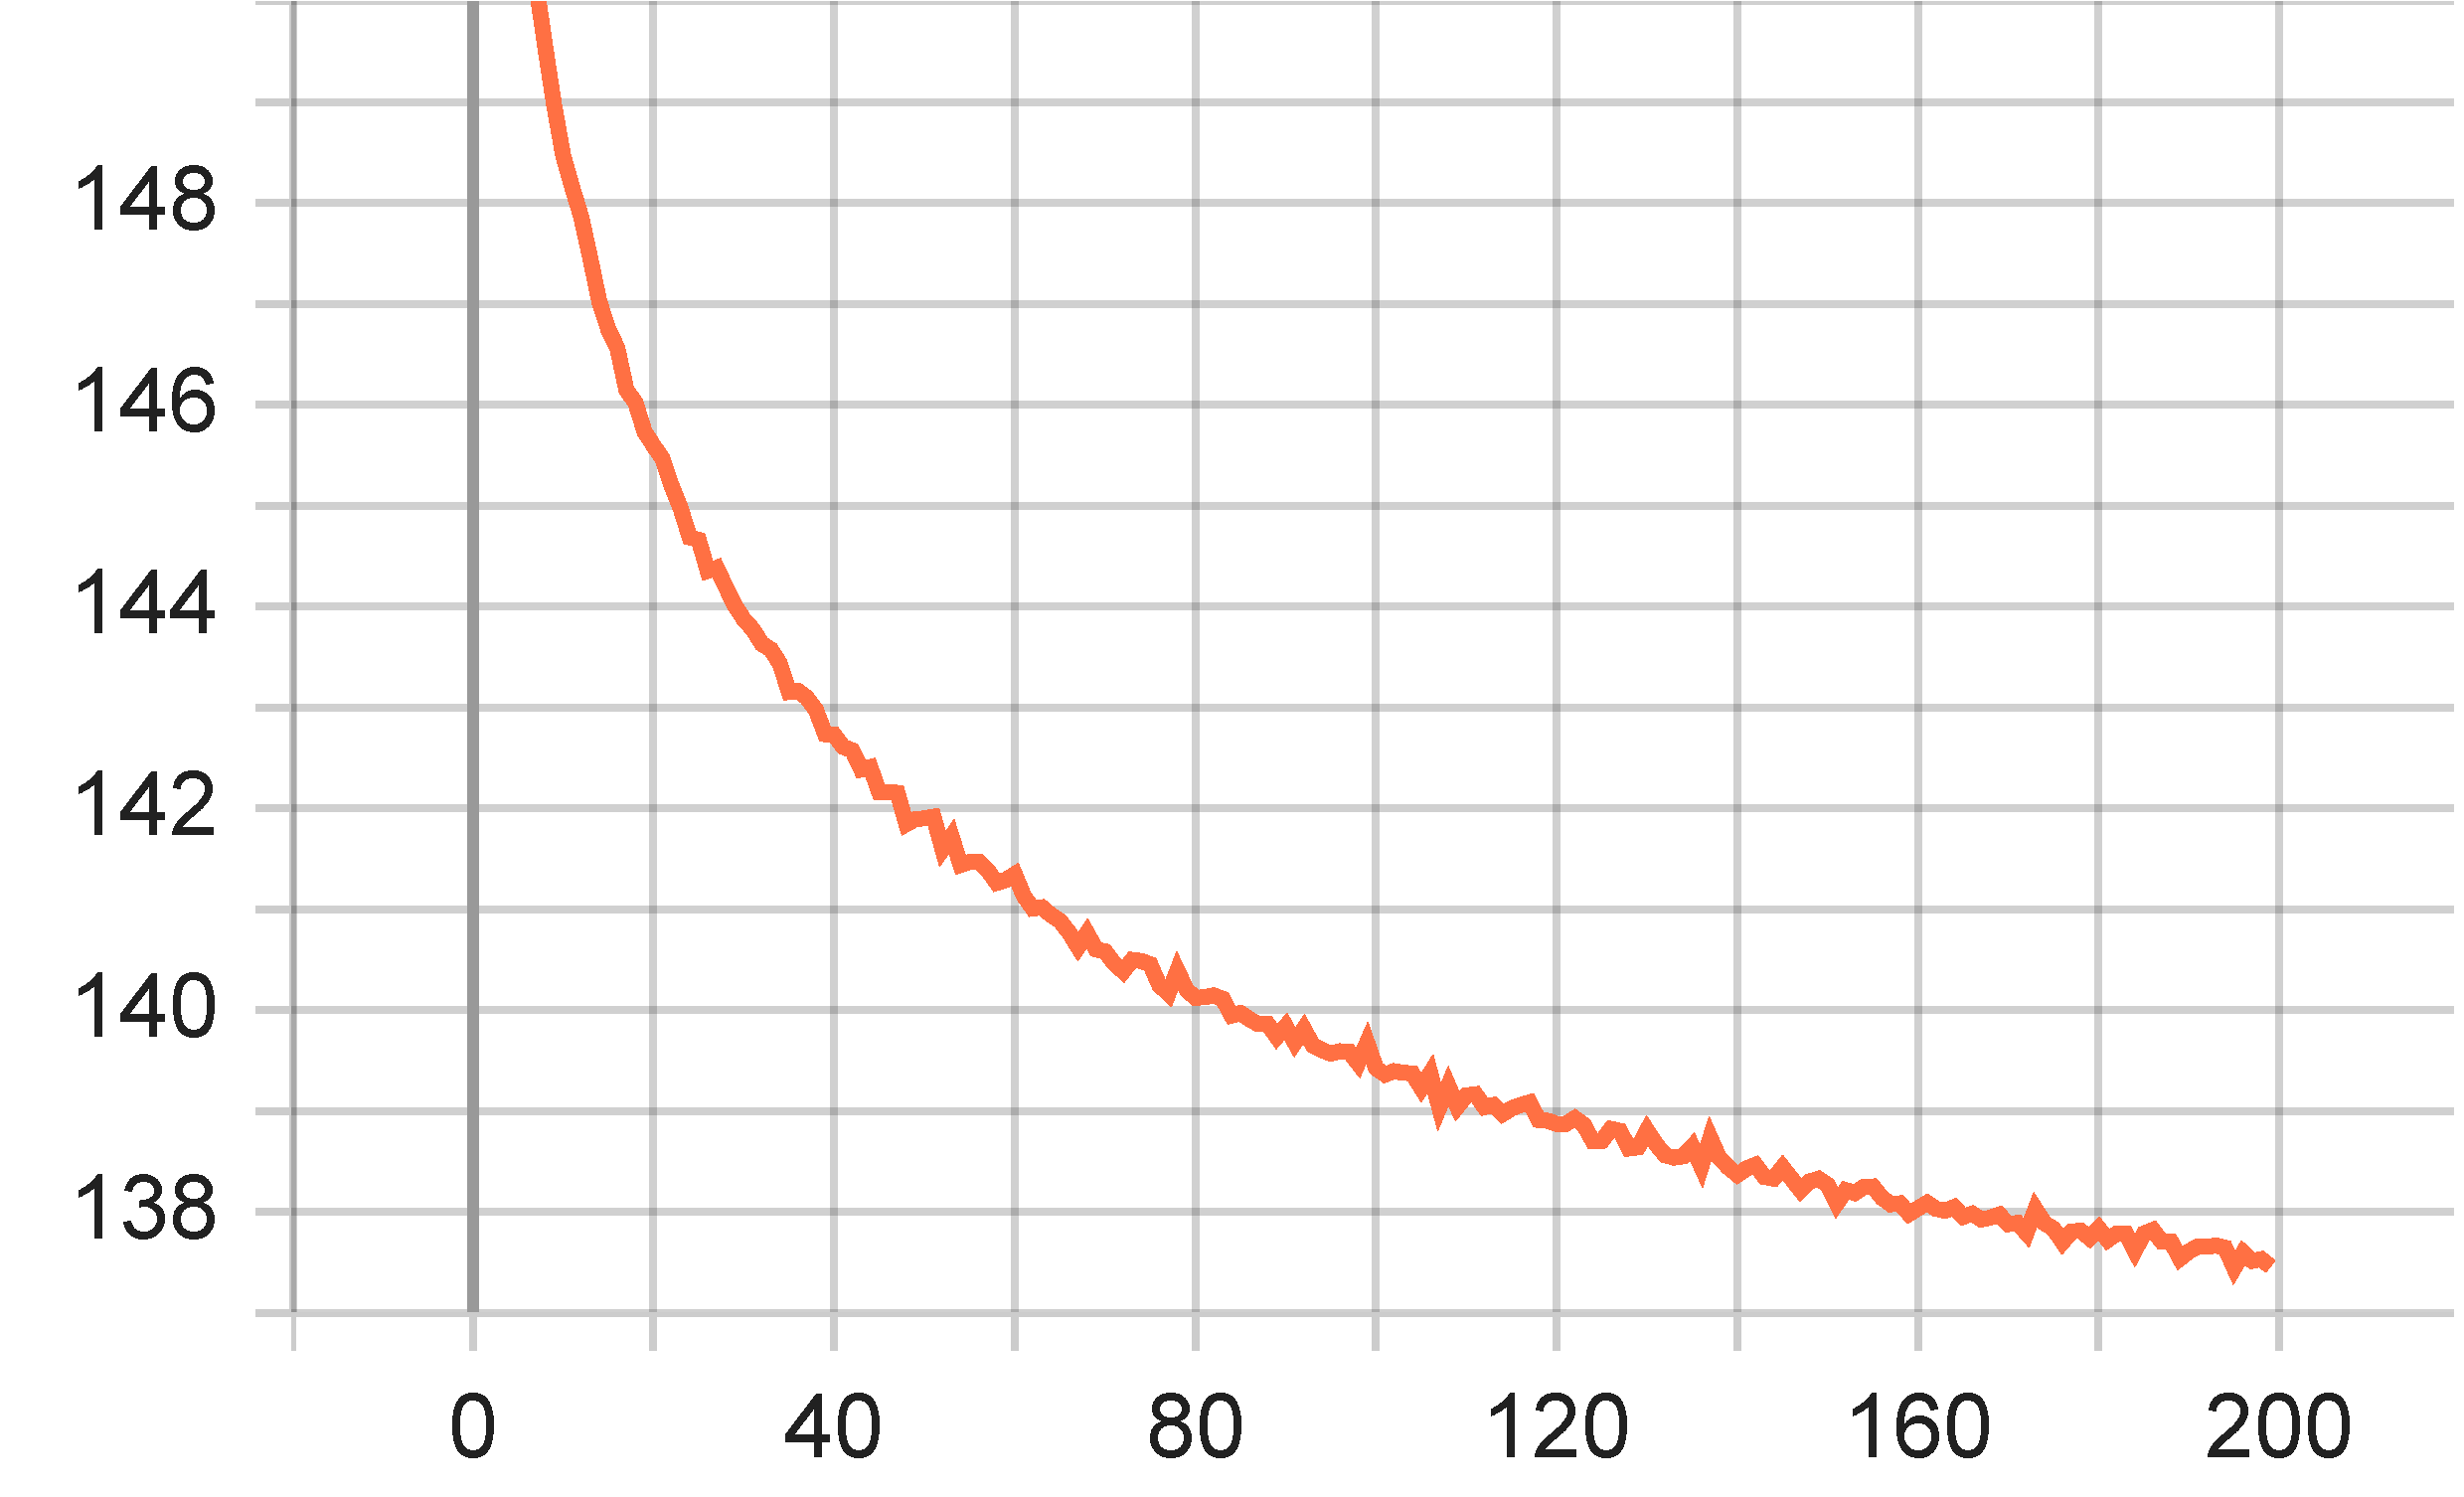
\includegraphics[width=0.97\textwidth]{figures/epoch_total_loss.pdf}
    \caption{Ztrátová funkce po 200 epochách konverguje k hodnotě $\sim 137.5$. Osa x značí počet epoch. Osa y značí hodnotu ztrátové funkce.}
\end{figure}

\begin{figure}[H]
    \centering
    \subfloat[\centering KL divergence po 200 epochách konverguje k hodnotě $\sim 3.79$.]{{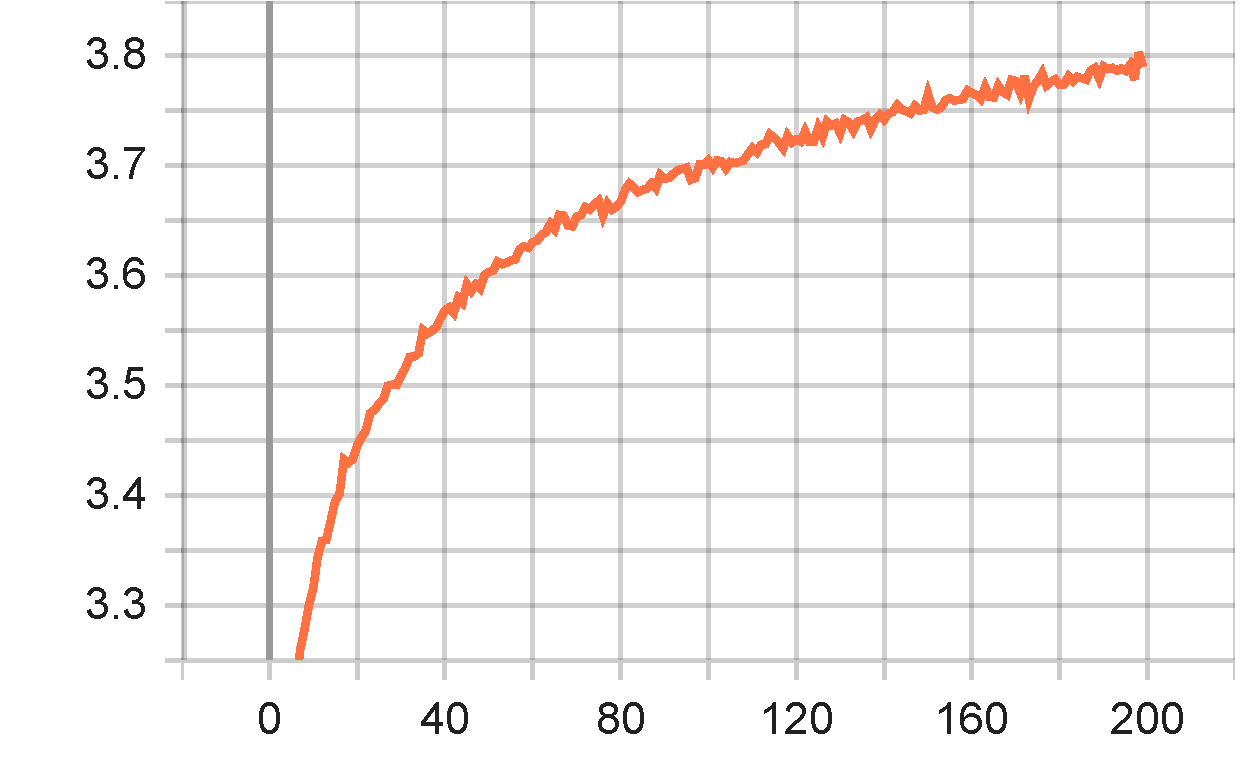
\includegraphics[width=0.45\textwidth]{figures/epoch_kl_loss.pdf} }}%
    \qquad
    \subfloat[\centering Chyba rekonstrukce po 200 epochách konverguje k hodnotě $\sim 133.7$.]{{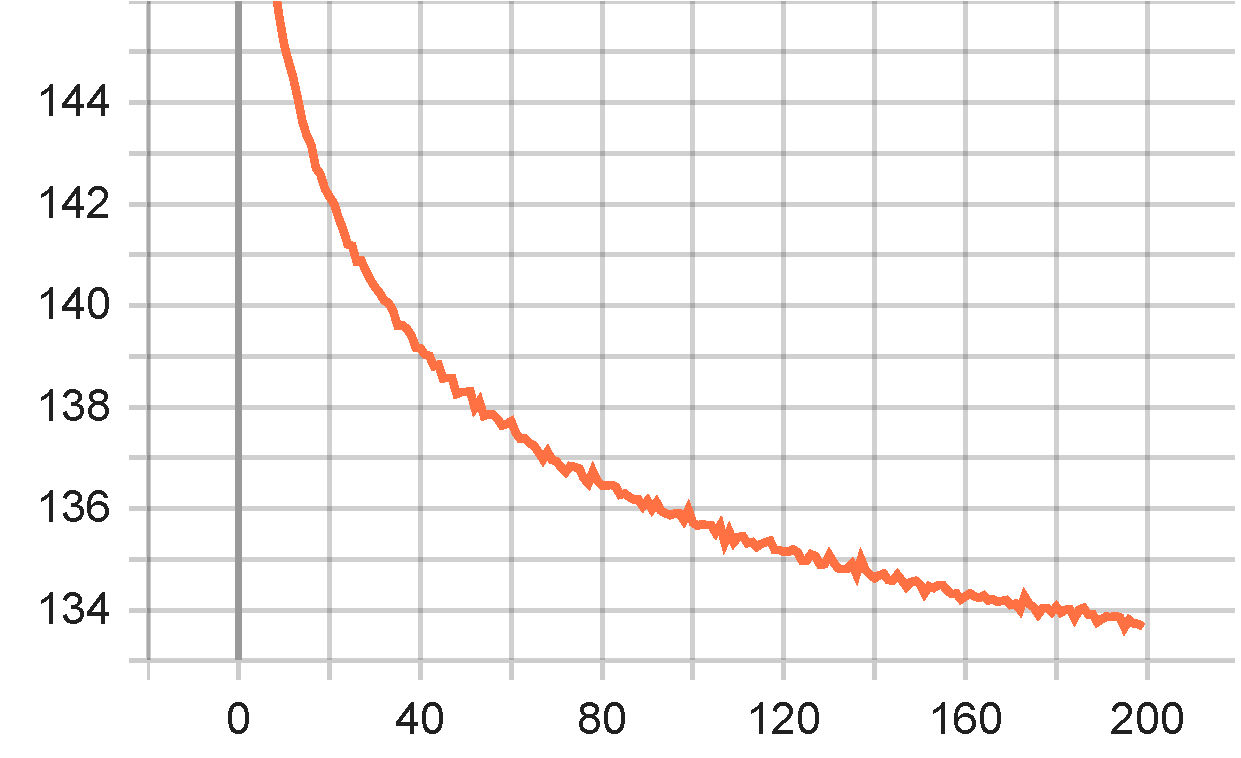
\includegraphics[width=0.45\textwidth]{figures/epoch_reconstruction_loss.pdf} }}%
    \caption{Hodnoty dílčích prvků ztrátové funkce modelu variačního autoenkodéru po 200 epochách. Osa x značí počet epoch. Osa y značí hodnotu dílčího prvku ztrátové funkce.}
    \label{fig:example}%
\end{figure}

Počet epoch byl na základě doménové znalosti (tedy předem známý počet tříd a sémantické vztahy mezi nimi) a postupného formování latentního prostoru, jak zachycuje \autoref{fig:forming_latent_space} stanoven na \textbf{500}.
Při vizualizaci latentního prostoru modelu, jehož trénovací fáze obsahovalo 500 epoch lze pozorovat emergenci struktury v latentní prostoru, která koresponduje se skutečným významem trénovacích dat (číslice 0-9, 10 skupin) a trénovací fáze tak v tomto bodě byla ukončena.